% --- CHAPTER 4: RESULTS AND EVALUATION ---
\chapter{Results and Evaluation}

\section{Experimental Results}
\label{sec:experimental_results}

This section demonstrates that the ConvCNP training procedure converges reliably and that the resulting model produces physically plausible downscaled predictions. Detailed quantitative evaluation follows in subsequent sections.

\subsection{Training Convergence}

\begin{figure}[H]
    \centering
    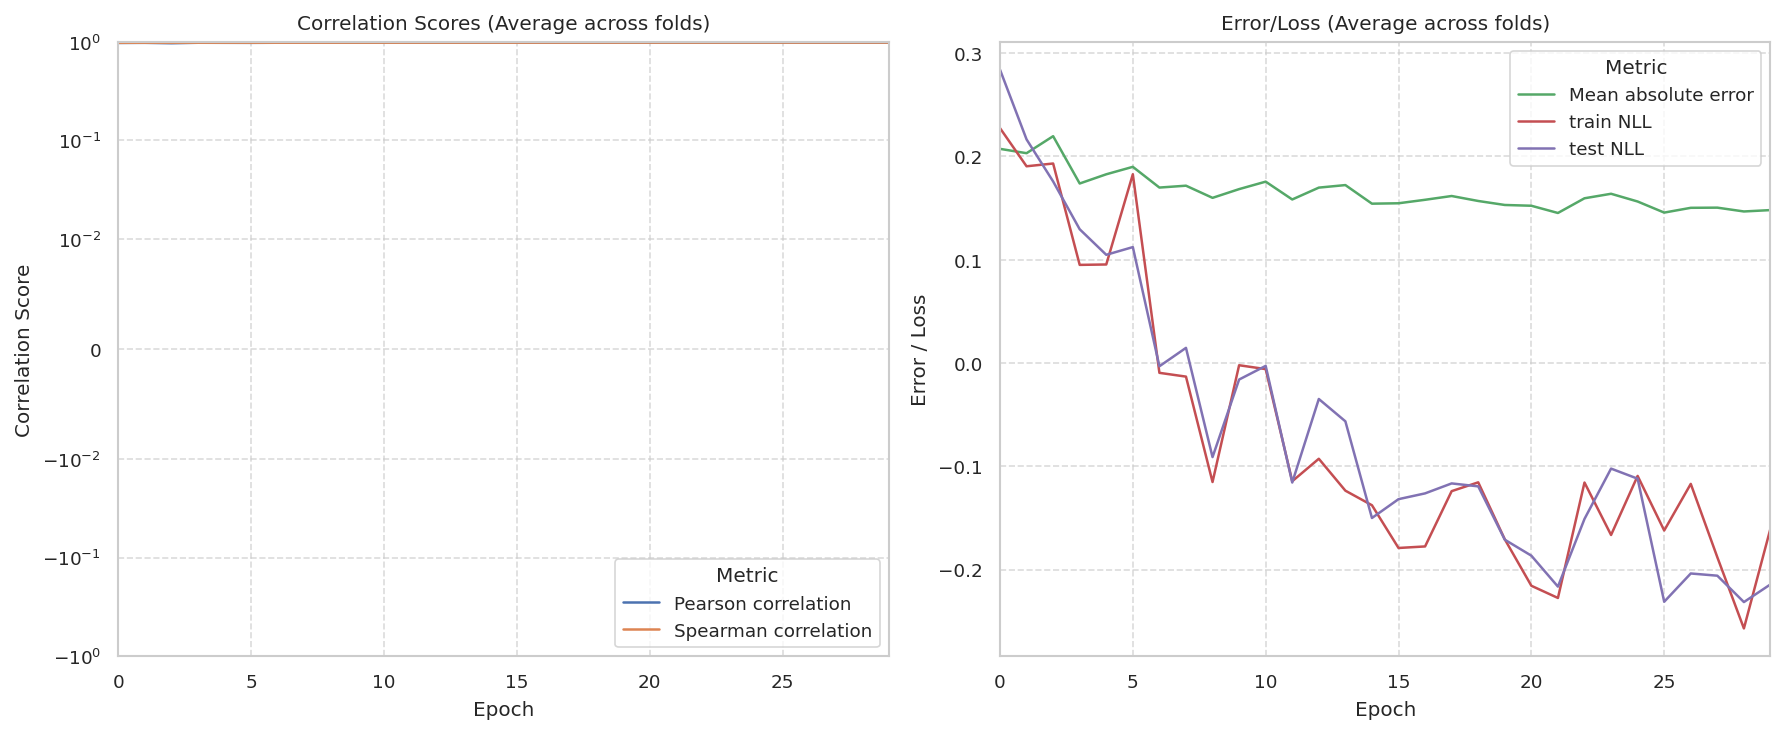
\includegraphics[width=\textwidth]{../trained_models/final-2014-30e-5f/trainingstats_all.png}
    \caption{Training curves for \texttt{final-2014-30e-5f}, averaged across five folds. Left: Pearson and Spearman correlations (log residual scale). Right: validation MAE (normalized units), training NLL, and validation NLL.}
    \label{fig:training_curves}
\end{figure}

Figure~\ref{fig:training_curves} shows the training curves for the primary ten-year model \newline (\texttt{final-2014-30e-5f}), averaged across all five cross-validation folds. The left panel tracks Pearson and Spearman correlation on a logarithmic residual scale ($1 - r$); the right panel shows the validation MAE (in normalized units) alongside the training and validation negative log-likelihood (NLL).


Three convergence trends are evident:

\begin{enumerate}
    \item \textbf{Error reduction.} The validation MAE drops steeply during the first five epochs---from ${\sim}0.21$ to ${\sim}0.16$ in normalized units---and continues to decrease more gradually thereafter, reaching ${\sim}0.14$ by epoch~30. All five folds exhibit the same pattern with tight variance: the best per-fold MAE values cluster around $0.141 \pm 0.001$, indicating consistent convergence.

    \item \textbf{Correlation improvement.} Both Pearson and Spearman correlations start high---above 0.967 already at epoch~0, reflecting the strong spatial structure in the temperature field---and improve to ${\sim}0.98$ by the end of training.

    \item \textbf{Loss decrease.} The training and validation NLL both decrease from positive values (${\sim}0.2$) to negative values (${\sim}{-}0.25$), indicating that the model learns to assign increasingly high likelihood to the observed targets. The two curves track each other closely throughout, with no divergence between them---a sign that overfitting is not occurring. No fold triggered early stopping; all five ran for the full 30~epochs, and the best checkpoints were selected between epochs~18 and~29, suggesting that marginal gains were still accumulating toward the end of training. This is further confirmed by the experiment running for up to 100 epochs (see below).
\end{enumerate}

\subsection{Sample Prediction}

\begin{figure}[H]
    \centering
    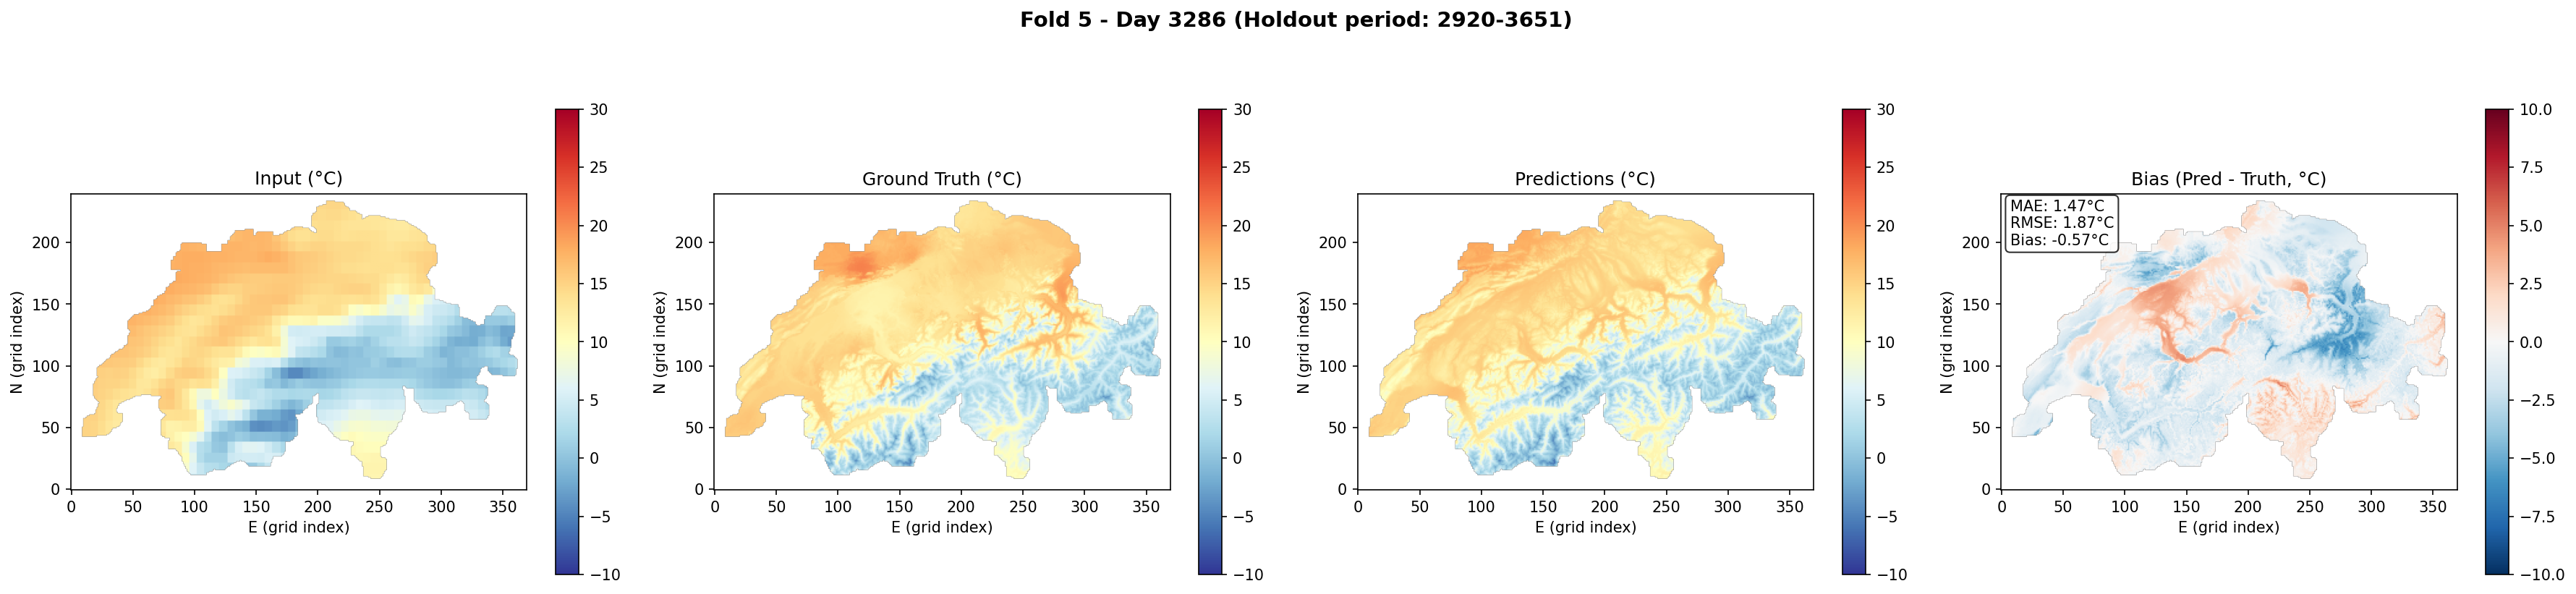
\includegraphics[width=\textwidth]{../trained_models/final-2014-30e-5f/plots/ERA5_GRID_PERCENT_1.0_fold4_prediction.png}
    \caption{Single-day prediction for fold~5 (day~3\,286) of the ten-year model. From left to right: ERA5-Land input (${\sim}$11\,km), MeteoSwiss ground truth (${\sim}$1\,km), model prediction (${\sim}$1\,km), and bias (prediction~$-$~truth). For this day and fold, MAE~=~1.47\,\textdegree C, RMSE~=~1.87\,\textdegree C, bias~=~$-$0.57\,\textdegree C.}
    \label{fig:sample_prediction}
\end{figure}

Figure~\ref{fig:sample_prediction} illustrates a single-day prediction from the fifth cross-validation fold.

The input panel shows the smooth, coarse-resolution temperature field from ERA5-Land, in which topographic detail is largely absent. The ground-truth panel reveals the fine-grained spatial structure that the model must recover: sharp temperature gradients along the Alpine ridge, cold mountain peaks, and warmer valleys---features well below the resolution of the input grid.

The prediction panel demonstrates that the model successfully reconstructs much of this detail. The overall spatial pattern closely follows the ground truth, with the major valleys, plateaus, and high-altitude regions clearly resolved. The bias panel confirms that residual errors are small across most of the domain (near-white shading), with the largest deviations concentrated in high-mountain areas where the elevation gradient is steepest.

\section{Performance}
\subsection{Global metrics}

Here are visualizations of the errors, error bias, CRPS and skill for the baseline model (10 years of data, 30 epochs, 5 folds, no ablation, aggregate results over the folds).

\begin{figure}[H]
    \centering
    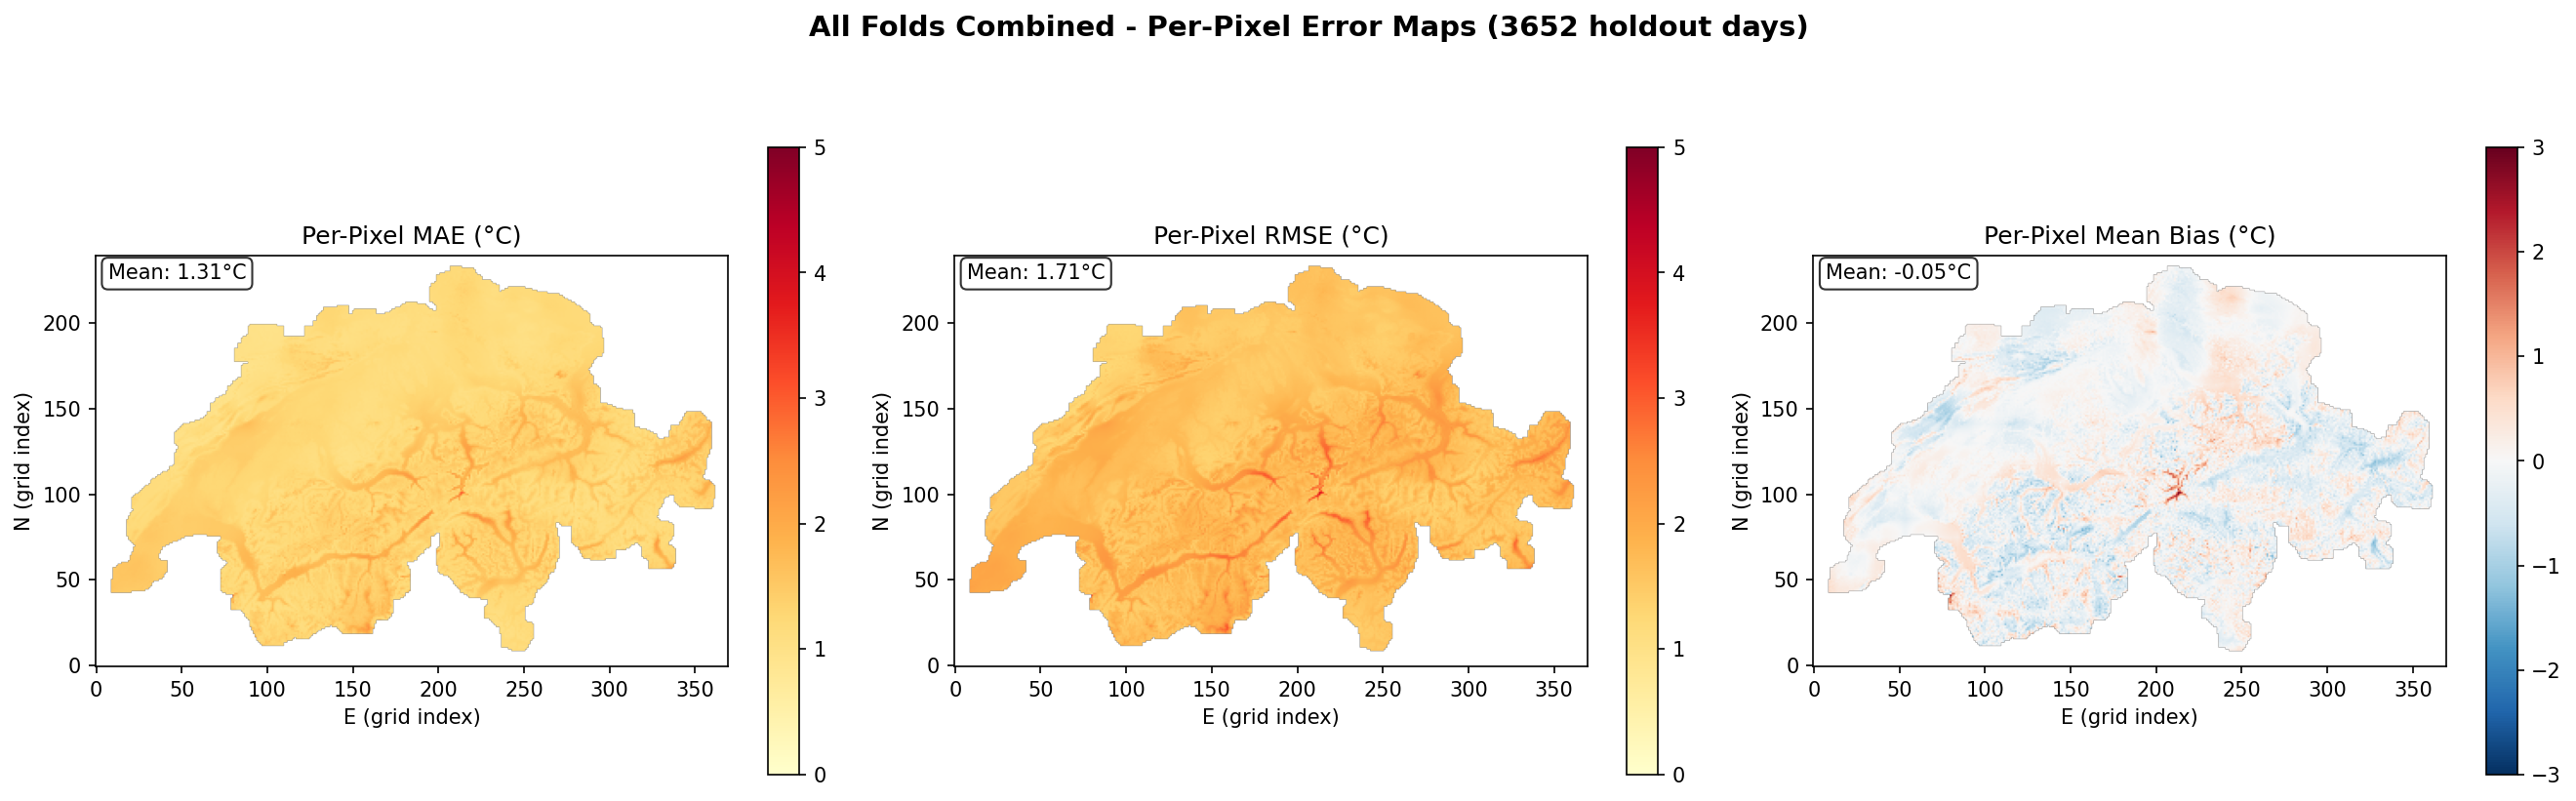
\includegraphics[width=\textwidth, trim={0 0 0 20px}, clip]{../trained_models/final-2014-30e-5f/plots/ERA5_GRID_PERCENT_1.0_error_maps.png}
    \caption{Per-pixel MAE, RMSE and error bias on maps}
    \label{fig:joint_error_maps}
\end{figure}

\begin{figure}[H]
    \centering
    \begin{tabular}{@{}cc@{}}
        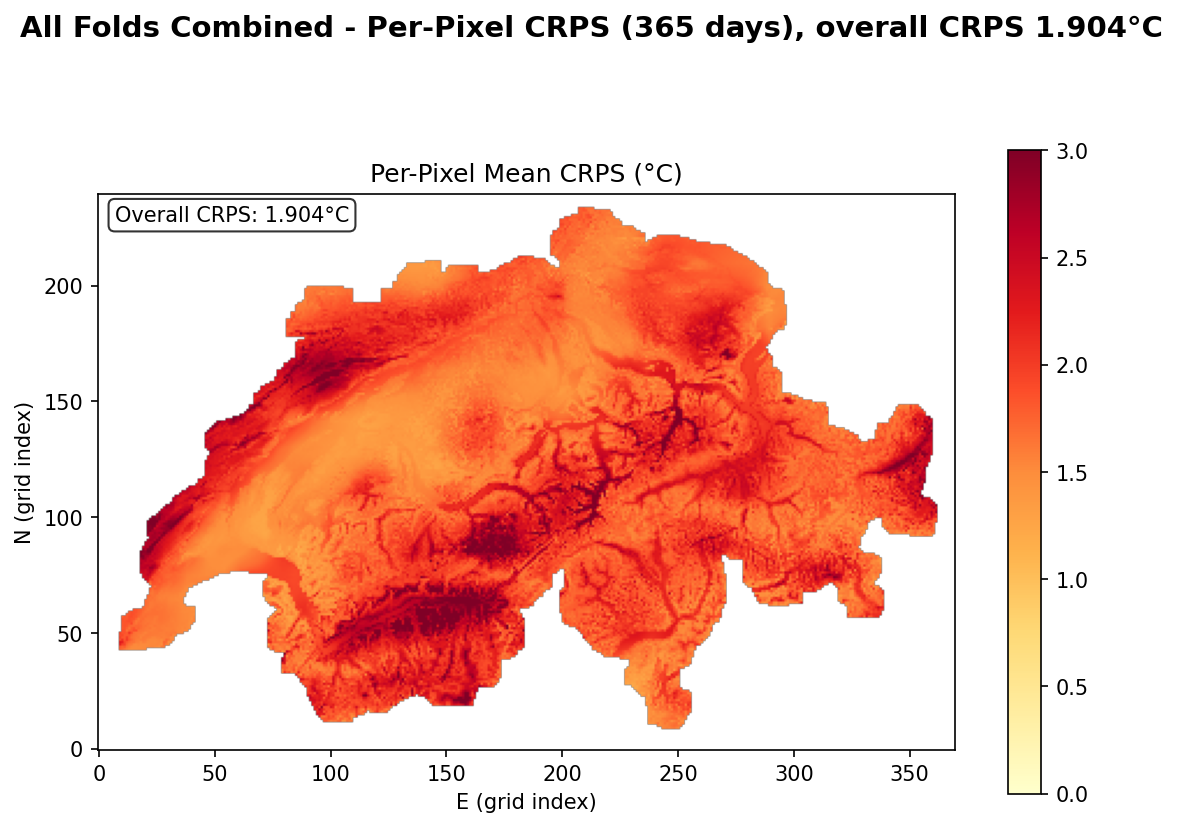
\includegraphics[width=0.48\textwidth, trim={0 0 0 25px}, clip]{../trained_models/final-2023-10e-5f/plots/ERA5_GRID_PERCENT_1.0_crps_map.png} &
        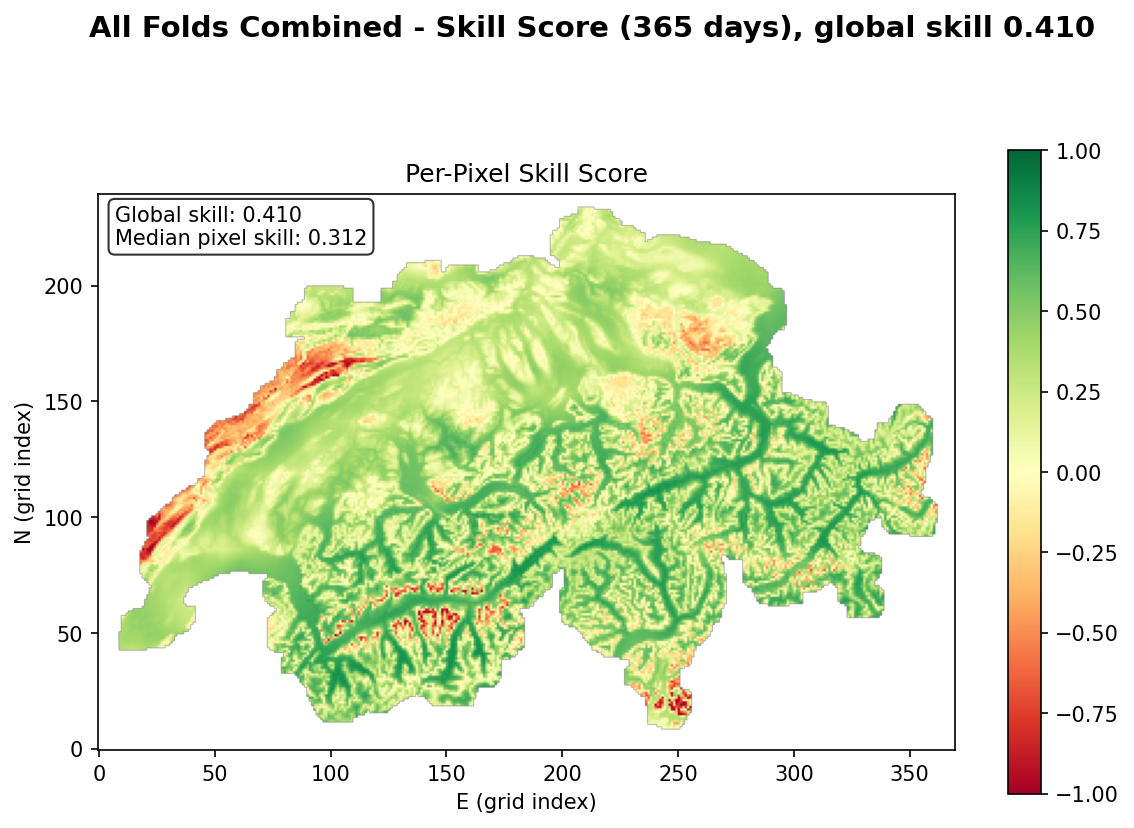
\includegraphics[width=0.48\textwidth, trim={0 0 0 25px}, clip]{../trained_models/final-2023-30e-5f/plots/ERA5_GRID_PERCENT_1.0_skill_map.png} \\
    \end{tabular}
    \caption{Per-pixel CRPS and Skill maps}
    \label{fig:qq_calibration}
\end{figure}

\begin{figure}[H]
    \centering
    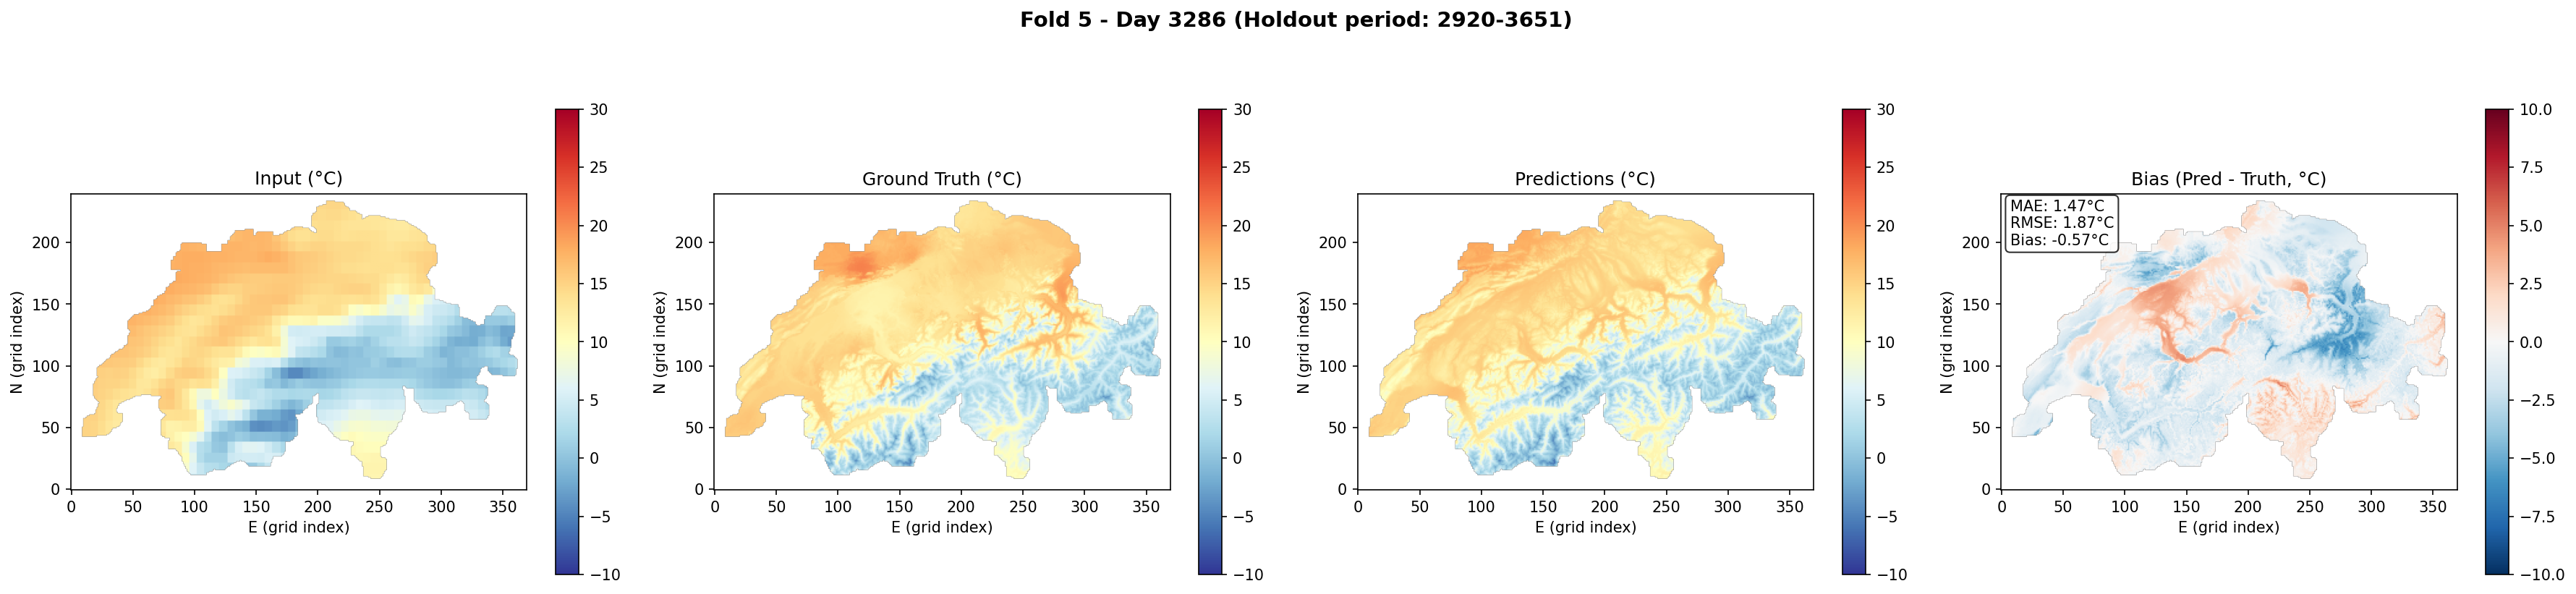
\includegraphics[width=\textwidth, trim={0 0 0 25px}, clip]{../trained_models/final-2014-30e-5f/plots/ERA5_GRID_PERCENT_1.0_fold4_prediction.png}
    \caption{Single-day prediction for fold~5 (day~3\,286) of the ten-year model. From left to right: ERA5-Land input (${\sim}$11\,km), MeteoSwiss ground truth (${\sim}$1\,km), model prediction (${\sim}$1\,km), and bias (prediction~$-$~truth). For this day and fold, MAE~=~1.47\,\textdegree C, RMSE~=~1.87\,\textdegree C, bias~=~$-$0.57\,\textdegree C.}
    \label{fig:sample_prediction}
\end{figure}

\begin{table}[H]
\centering
\caption{Full-grid evaluation overview. All models evaluated with 100\% of the ERA5-Land grid (1\,769~points) as context input.}
\label{tab:full_grid_overview}
\begin{tabular}{@{}lrrrrr@{}}
\toprule
\textbf{Model} & \textbf{MAE} & \textbf{RMSE} & \textbf{Bias} & \textbf{CRPS} & \textbf{Skill} \\
                & (\textdegree C) & (\textdegree C) & (\textdegree C) & (\textdegree C) & \\
\midrule
\multicolumn{6}{@{}l}{\textit{Primary models}} \\
\quad \texttt{2023-10e-5f}   & 2.09 & 2.67 & $+$0.66 & 1.90 & 0.245 \\
\quad \texttt{2023-30e-5f}   & 1.64 & 2.08 & $+$0.24 & 1.49 & 0.410 \\
\quad \texttt{2023-100e-5f}  & 1.62 & 2.05 & $+$0.25 & 1.48 & 0.415 \\
\quad \texttt{2014-30e-5f}  (base model)   & 1.31 & 1.71 & $-$0.05 & 1.21 & 0.524 \\
\midrule
\bottomrule
\end{tabular}
\end{table}

\newpage
Table~\ref{tab:full_grid_overview} summarises the headline accuracy and skill metrics for all evaluated models on the full ERA5-Land grid (1\,769 context points). Each row reports the mean absolute error (MAE), root-mean-square error (RMSE), and mean bias of the point prediction in degrees Celsius, together with the Continuous Ranked Probability Score (CRPS) and a skill score defined as $\text{Skill} = 1 - \text{CRPS}_{\text{model}} / \text{CRPS}_{\text{ref}}$, where the reference is the deterministic bilinear interpolation of ERA5-Land to the target grid (for a deterministic forecast, $\text{CRPS} = \text{MAE}$). A skill of~0 indicates no improvement over the interpolation baseline; a skill of~1 would indicate a perfect forecast.

\paragraph{Effect of training duration.}
The three single-year models (trained on 2023 data, evaluated on 365 holdout days) isolate the effect of longer optimisation. Increasing from 10 to 30~epochs cuts the MAE from 2.09 to 1.64\,\textdegree C (a 22\% reduction) and nearly doubles the skill score from 0.245 to 0.410. Extending training further to 100~epochs yields only a marginal additional gain (MAE 1.62\,\textdegree C, Skill 0.415), suggesting that most of the representational capacity available to the single-year model is utilised within the first 30~epochs. Even though the slowdown was found, up to 100 epochs convergence continues without signs of overfitting.

\paragraph{Effect of training data volume.}
Moving from one year to ten years of training data (both at 30~epochs) produces the largest single improvement: the MAE drops from 1.64 to 1.31\,\textdegree C, the RMSE from 2.08 to 1.71\,\textdegree C, and the skill score rises from 0.410 to 0.524. The mean bias also shrinks to near zero ($-$0.05\,\textdegree C). These gains indicate that additional climatological diversity---exposing the model to a wider range of synoptic situations and seasonal extremes---is more beneficial than additional gradient steps on a limited sample.

\paragraph{Skill relative to ERA5-Land interpolation.}
All primary models improve upon the bilinear-interpolation baseline. The ten-year model achieves a CRPS-based skill of 0.524, meaning its probabilistic predictions reduce the expected error by more than half compared to simply interpolating the coarse reanalysis field. Even the weakest model (10~epochs, single year) attains a skill of 0.245, confirming that the ConvCNP learns meaningful fine-scale structure beyond what spatial interpolation alone can provide.

\paragraph{Uncertainty calibration.}
\nopagebreak
\begin{figure}[H]
    \centering
    \begin{tabular}{@{}cc@{}}
        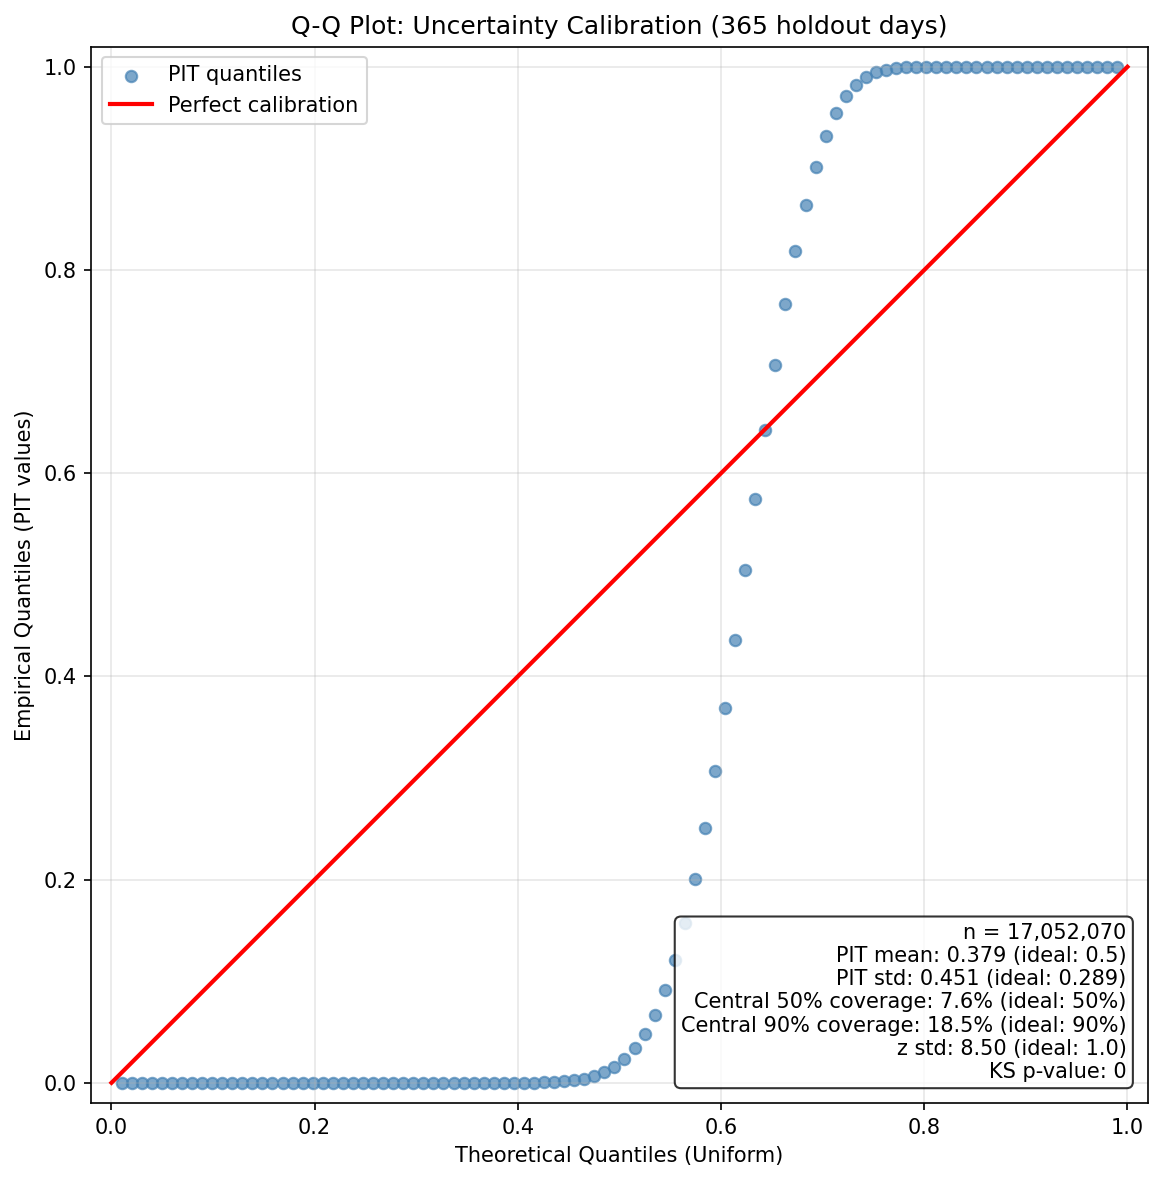
\includegraphics[width=0.48\textwidth]{../trained_models/final-2023-10e-5f/plots/ERA5_GRID_PERCENT_1.0_qq_calibration.png} &
        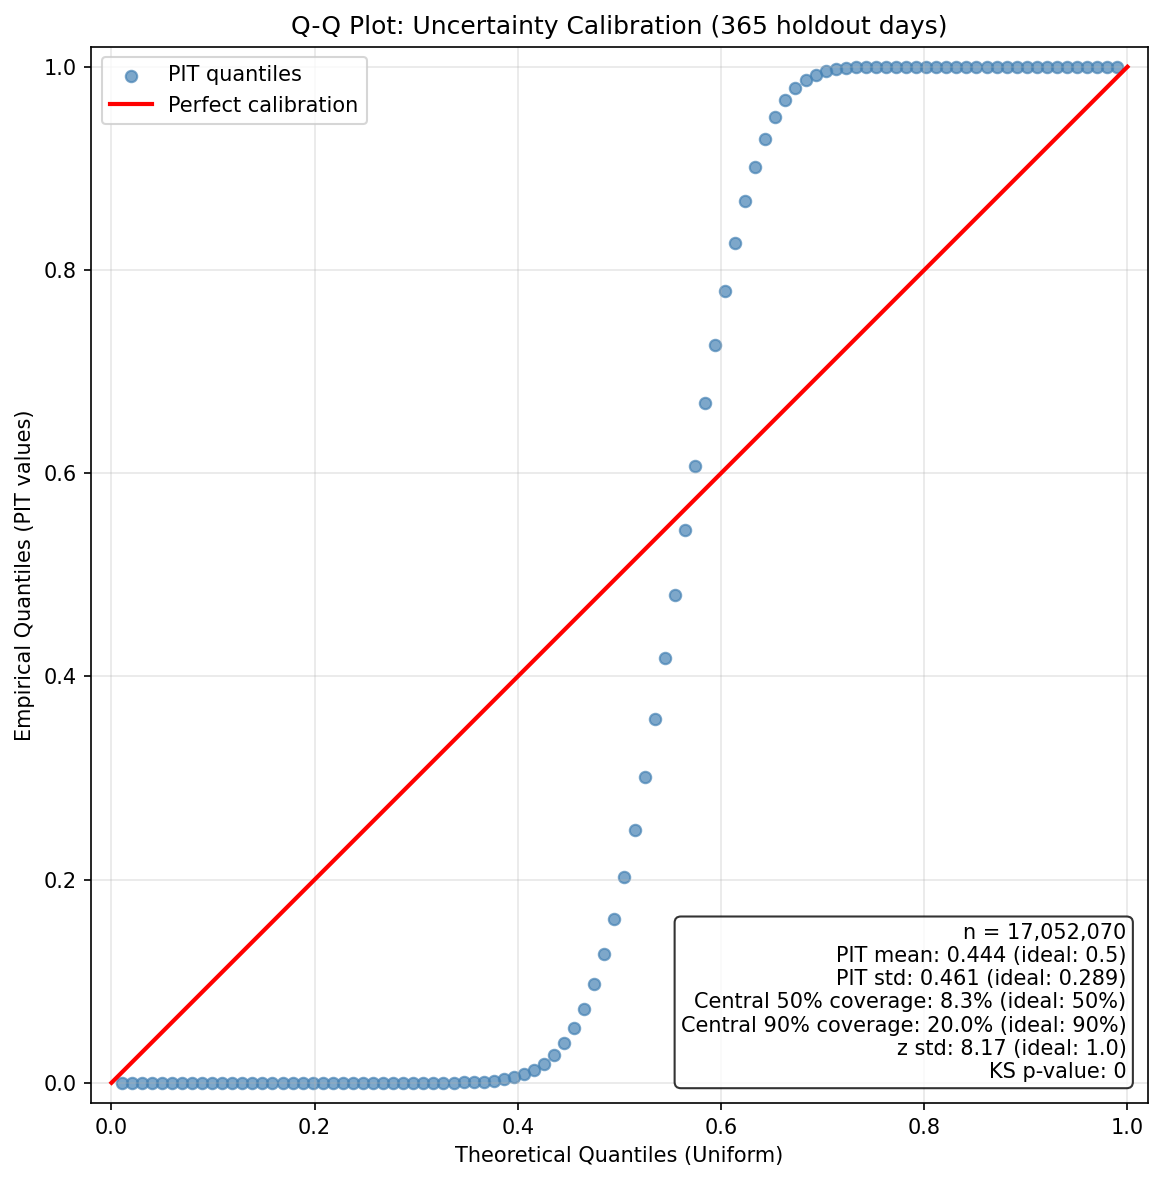
\includegraphics[width=0.48\textwidth]{../trained_models/final-2023-30e-5f/plots/ERA5_GRID_PERCENT_1.0_qq_calibration.png} \\
        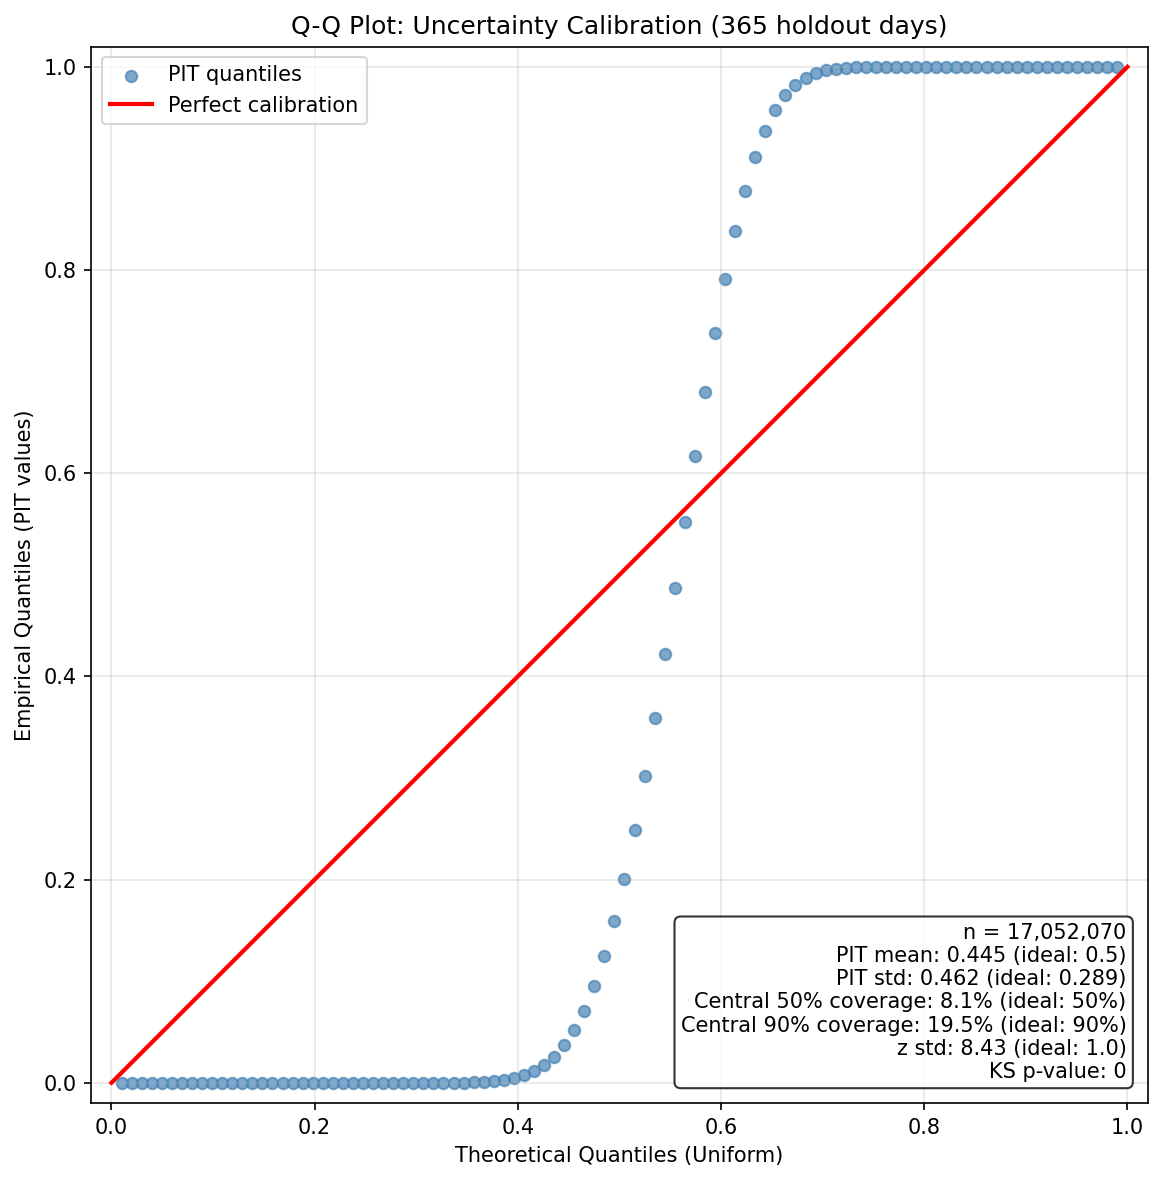
\includegraphics[width=0.48\textwidth]{../trained_models/final-2023-100e-5f/plots/ERA5_GRID_PERCENT_1.0_qq_calibration.png} &
        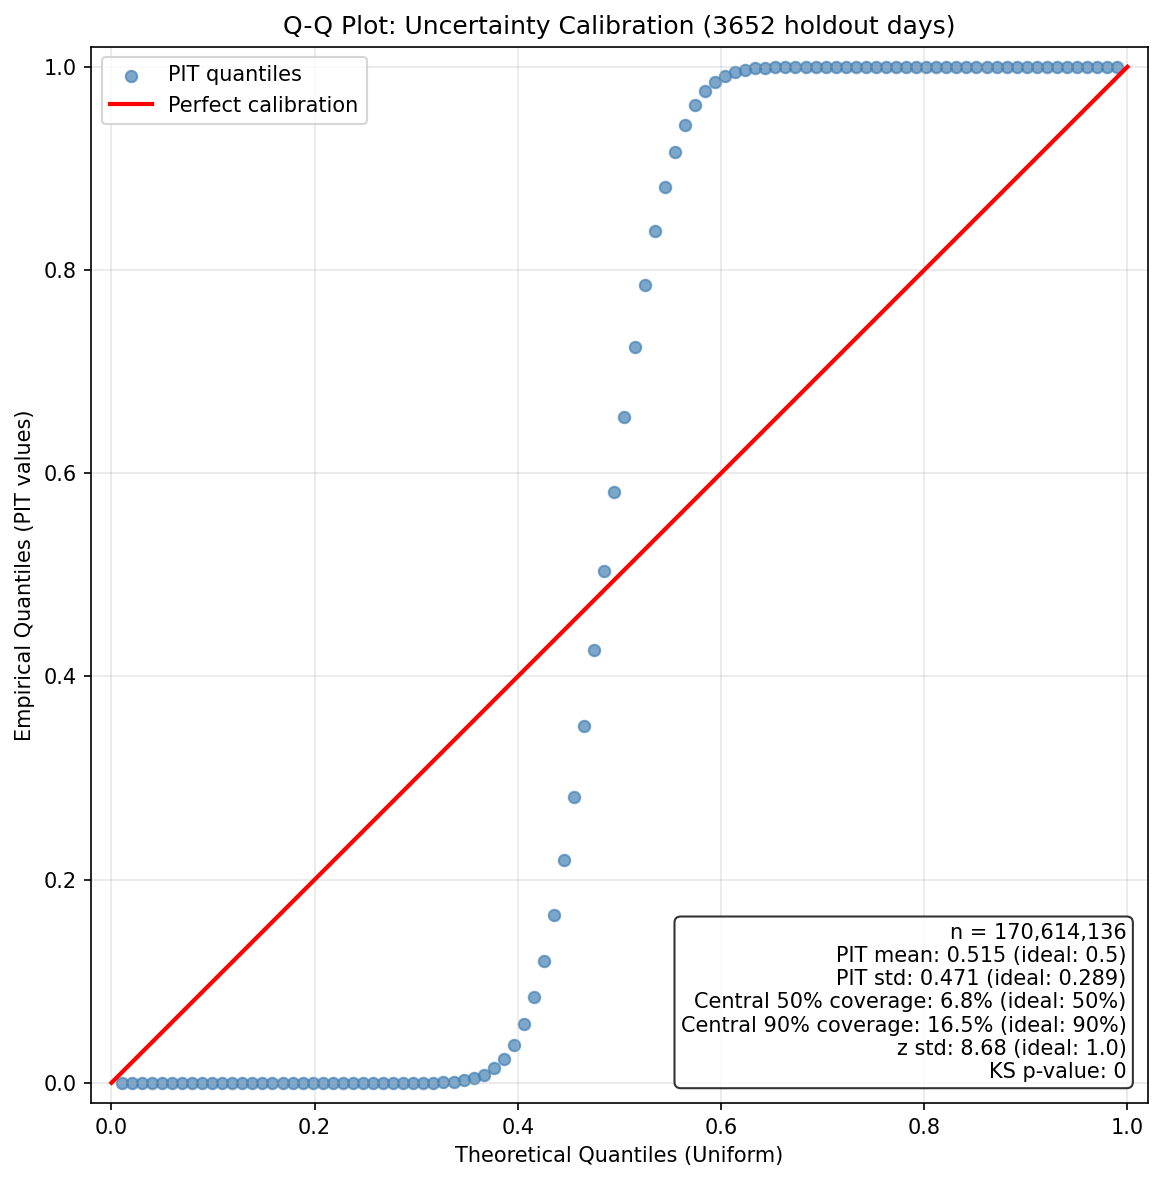
\includegraphics[width=0.48\textwidth]{../trained_models/final-2014-30e-5f/plots/ERA5_GRID_PERCENT_1.0_qq_calibration.png} \\
    \end{tabular}
    \caption{Q--Q calibration plots (PIT quantiles vs.\ uniform theoretical quantiles) for the four primary models. Top row: single-year models at 10 and 30~epochs. Bottom row: single-year model at 100~epochs (left) and ten-year model at 30~epochs (right). All models are substantially overconfident, with central 90\% coverage ranging from 16.5\% to 20\%.}
    \label{fig:qq_calibration}
\end{figure}

Figure~\ref{fig:qq_calibration} shows Q--Q plots of the Probability Integral Transform (PIT) for each primary model. A perfectly calibrated model would produce PIT values uniformly distributed on $[0,1]$, yielding points along the diagonal. All four models exhibit a pronounced S-shaped departure: the empirical quantiles rise steeply, the standardised residual standard deviation ($z$-std) is approximately 8.7 (ideal: 1.0), confirming that the model is overconfident by roughly an order of magnitude.

This miscalibration is consistent across all configurations and may arise from the Gaussian likelihood training objective, which optimises overall fit rather than interval coverage. 

\subsection{Correlations}

\begin{figure}[H]
    \centering
    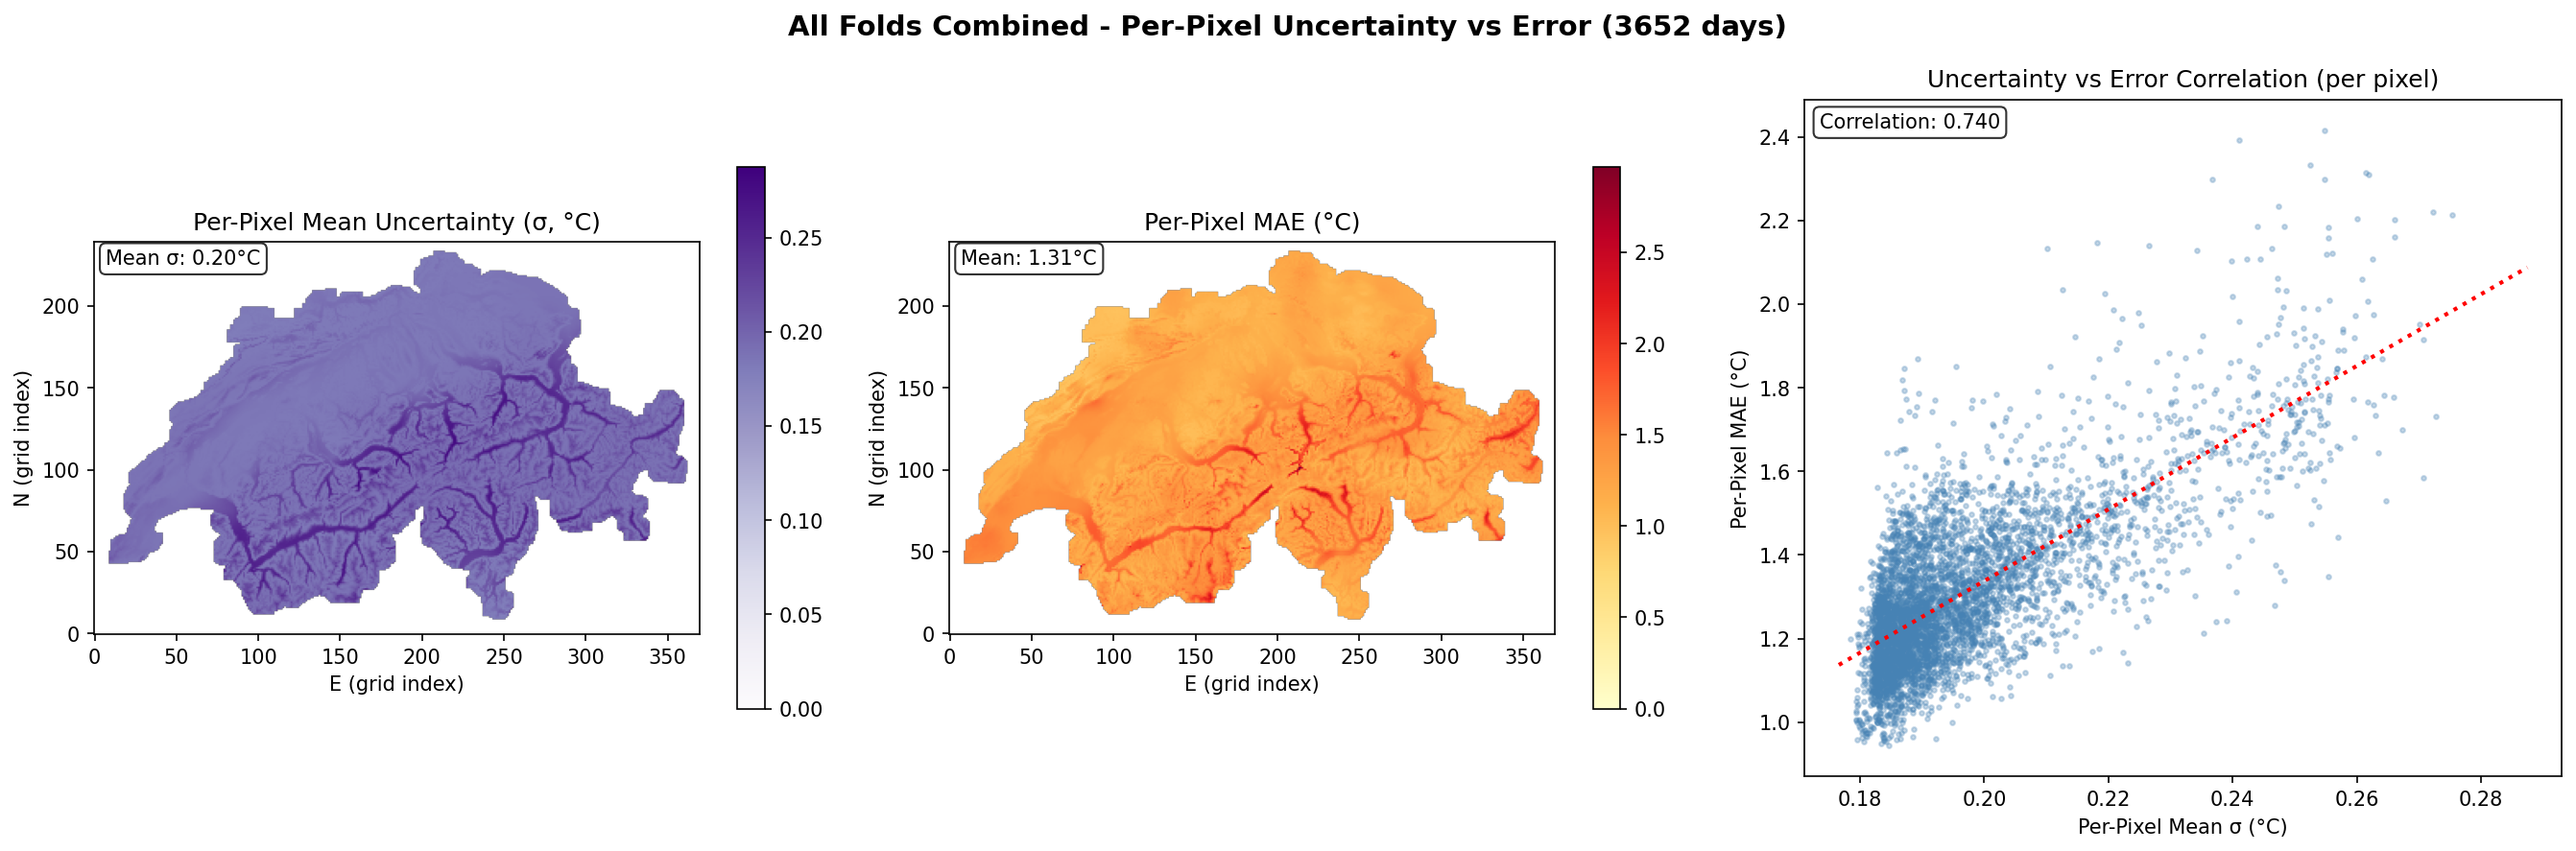
\includegraphics[width=\textwidth, trim={0 0 0 25px}, clip]{../trained_models/final-2014-30e-5f/plots/ERA5_GRID_PERCENT_1.0_uncertainty_vs_error.png}
    \caption{Uncertainty map, error map for comparison, and cross-correlation on the baseline model, covering 10 years of training data, 30 epochs, 5 folds, no ablation, conjoined results from all folds.}
    \label{fig:sample_prediction}
\end{figure}

Despite the overconfidence mentioned above, the model's predicted uncertainties remain informative: the correlation between predicted $\sigma$ and absolute error is 0.74 for the ten-year model, meaning that the uncertainty estimates reliably rank predictions by quality even though their absolute magnitudes are too small.

\begin{figure}[H]
    \centering
    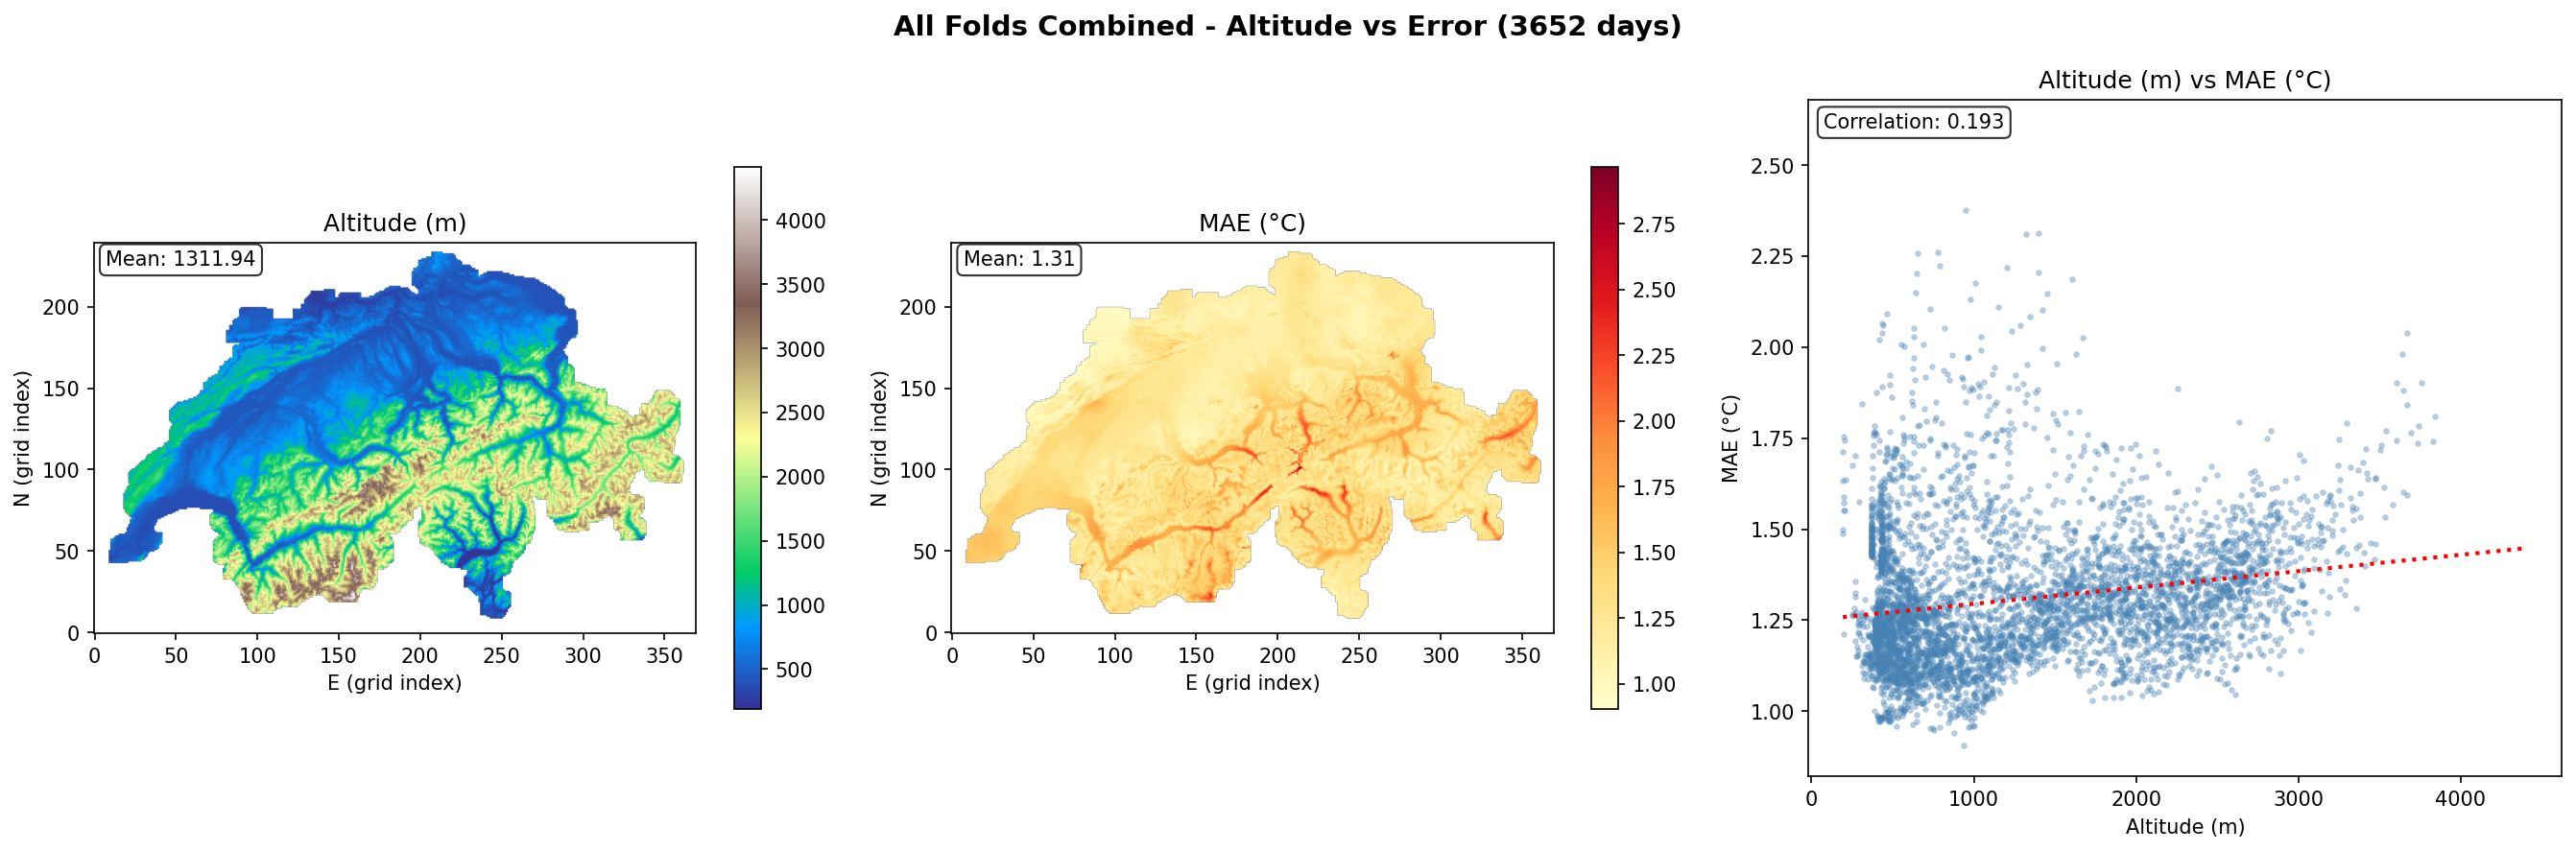
\includegraphics[width=\textwidth, trim={0 0 0 25px}, clip]{../trained_models/final-2014-30e-5f/plots/ERA5_GRID_PERCENT_1.0_altitude_vs_error.png}
    \caption{Altitude map, error map for comparison, and cross-correlation on the baseline model, covering 10 years of training data, 30 epochs, 5 folds, no ablation, conjoined results from all folds.}
    \label{fig:sample_prediction}
\end{figure}

It is known that weather prediction at altitude is a tough problem. The correlation between altitude and error exists, but is significantly lower.

\begin{figure}[H]
    \centering
    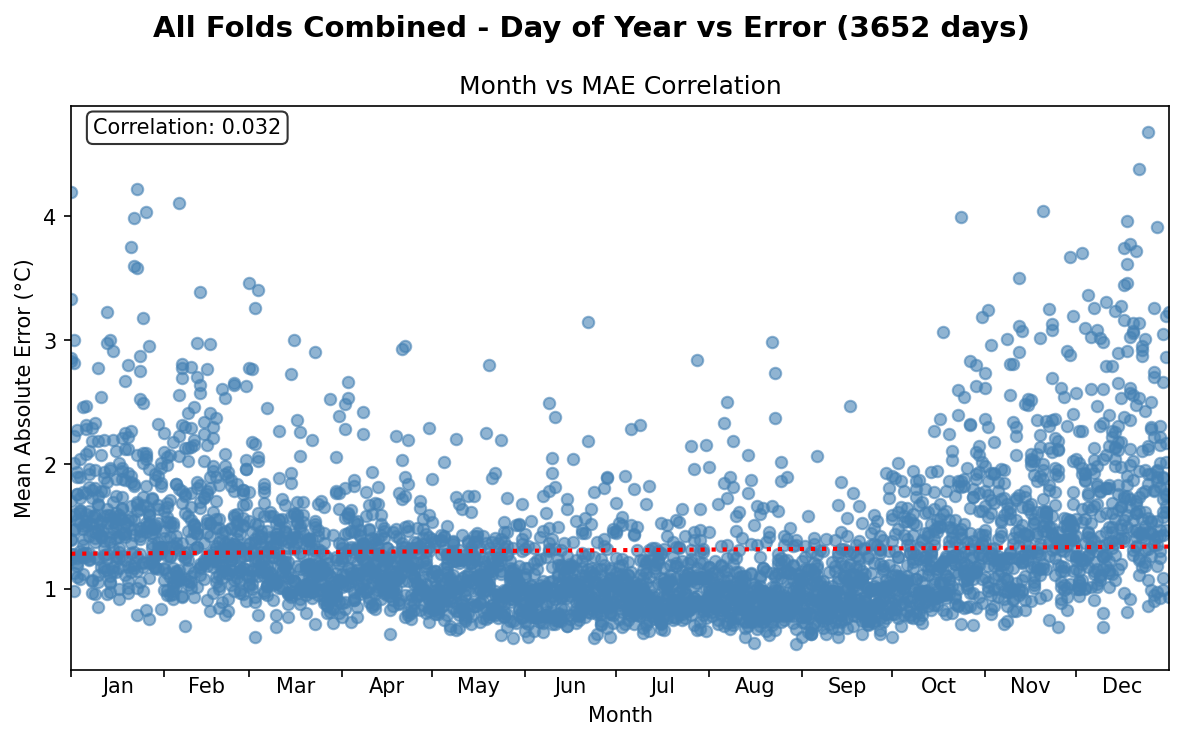
\includegraphics[width=\textwidth, trim={0 0 0 25px}, clip]{../trained_models/final-2014-30e-5f/plots/ERA5_GRID_PERCENT_1.0_doy_vs_error.png}
    \caption{Mean error per day-of-year, covering 10 years of training data, 30 epochs, 5 folds, no ablation, conjoined results from all folds.}
    \label{fig:sample_prediction}
\end{figure}

We can observe the colder months (November--March) observe a higher incidence of outliers in mean absolute error.


\section{Ablation Analysis}
\label{sec:ablation}

\begin{table}[H]
\centering
\caption{Full-grid evaluation overview. All models evaluated with 100\% of the ERA5-Land grid (1\,769~points) as context input.}
\label{tab:full_grid_overview}
\begin{tabular}{@{}lrrrrr@{}}
\toprule
\textbf{Model} & \textbf{MAE} & \textbf{RMSE} & \textbf{Bias} & \textbf{CRPS} & \textbf{Skill} \\
                & (\textdegree C) & (\textdegree C) & (\textdegree C) & (\textdegree C) & \\
\midrule
\multicolumn{6}{@{}l}{\textit{Primary model (2014--2023)}} \\
\quad \texttt{2014-30e-5f}  (base model)   & 1.31 & 1.71 & $-$0.05 & 1.21 & 0.524 \\
\midrule
\multicolumn{6}{@{}l}{\textit{Ablation models (2014--2023)}} \\
\quad \texttt{-ablation-elevation}\textsuperscript{$\dagger$}
                              & \multicolumn{5}{c}{--- model diverged; see text ---} \\
\quad \texttt{-ablation-mtpi}            & 1.33 & 1.74 & $-$0.13 & 1.23 & 0.517 \\
\makecell[l]{\quad \texttt{-ablation-seasonal-all} \textsuperscript{$\ddagger$} \\ \quad \quad (suggest discarding)} & 1.29 & 1.69 & $+$0.08 & 1.19 & 0.532 \\
\quad \texttt{-ablation-seasonal-in-mlp}\textsuperscript{$\ddagger$}
                                         & 1.29 & 1.69 & $+$0.08 & 1.19 & 0.532 \\
\bottomrule
\end{tabular}
\begin{flushleft}
\textsuperscript{$\dagger$}\small Without the elevation MLP, the model produced errors orders of magnitude above physical plausibility (MAE~$\approx$~802\,\textdegree C), indicating that the topographic correction stage is essential for meaningful predictions. (This is unexpected, we would expect some degree of interpolation to still take place.) \\[2pt]
\textsuperscript{$\ddagger$}\small These two ablations produced bit-identical metrics across all evaluation categories, despite differing in whether seasonal features are present in the CNN input - this is discussed below. Surprisingly, both of them present a higher skill than the base model.
\end{flushleft}
\end{table}

All ablation models use the same ten-year dataset (2014--2023), 30 training epochs, five-fold cross-validation, and identical splits as the base model. Each experiment disables a single feature group while keeping everything else unchanged, so that differences in the metrics can be attributed to that component alone.

\paragraph{Elevation features.}
Removing the three topographic inputs---true elevation, elevation difference, and TPI---from the elevation MLP (\texttt{USE\_ELEVATION=False}) caused the model to diverge catastrophically. The resulting MAE of ${\sim}802$\,\textdegree C and a negative skill score of $-314$ indicate that the predictions are off-scale by orders of magnitude. Notably, the altitude--error correlation jumps from 0.19 in the base model to 0.78 in this ablation, confirming that the errors are overwhelmingly concentrated at locations where the true elevation differs most from the coarse ERA5-Land grid-cell elevation. Without topographic correction, the elevation MLP receives only the CNN's interpolated $(\mu, \sigma)$ and zero-valued placeholders; it has no mechanism to compensate for the fact that a 3\,000\,m peak and a 400\,m valley within the same ${\sim}$11\,km grid cell receive nearly identical CNN predictions. The MLP, trained on these uninformative inputs, learns weight configurations that produce numerically unstable outputs at evaluation time---when all 46\,000+ target points are predicted simultaneously---resulting in the observed divergence. This outcome confirms that the elevation MLP is not merely a refinement stage but the \emph{essential} component that bridges the resolution gap between the coarse reanalysis grid and the fine-scale target field. The author must also consider that there may have been some misconfiguration or bug which could cause this, but one was not identified.

\paragraph{Topographic Position Index.}
Removing only the TPI channel \newline (\texttt{USE\_MTPI=False}) while retaining true elevation and elevation difference has a marginal effect: the MAE increases from 1.31 to 1.33\,\textdegree C and the skill score decreases from 0.524 to 0.517. The bias shifts from $-0.05$ to $-0.13$\,\textdegree C, a small systematic cold bias. This suggests that TPI---which encodes whether a target lies on a ridge, in a valley, or on an open slope---provides a secondary, but not essential, correction on top of the elevation difference. The elevation difference alone captures most of the sub-grid topographic variance.

\paragraph{Seasonal features.}
Two ablations target the cyclical day-of-year encoding ($\cos$/$\sin$ channels). The first (\texttt{-ablation-seasonal-all}) removes them everywhere: both from the CNN input channels and from the elevation MLP. The second \newline (\texttt{-ablation-seasonal-in-mlp}) removes them only from the MLP while keeping them in the CNN input. Both produce \emph{bit-identical} metrics: MAE\,=\,1.29\,\textdegree C, Skill\,=\,0.532.

This identity means the CNN learns to completely ignore the explicit seasonal channels in its input. While the temperature field itself carries seasonal information, it is very noisy and goes not offer a reliable gradient. This suggests that \texttt{USE\_SEASONAL=False} might possibly not be wired correctly. We therefore suggest discarding that ablation model from our analysis.

\paragraph{Seasonal ablations from the MLP outperform the base model.}
Counter-intuitively, this ablation achieve slightly \emph{better} metrics than the base model (MAE 1.29 vs.\ 1.31\,\textdegree C; Skill 0.532 vs.\ 0.524). The improvement is small but consistent across all metrics. This likely reflects a mild regularisation effect: the base model's elevation MLP has 7~inputs (including $\cos$/$\sin$), while the seasonal ablations have only 5, reducing the MLP's capacity to overfit to spurious correlations between the seasonal encoding and the residual error. Alternatively, feeding redundant features to the MLP may slightly impede optimisation by diluting the gradient signal from the more informative elevation inputs. In either case, the practical difference is modest, and the result suggests that removing the explicit seasonal features is, if anything, slightly beneficial. This also suggests the MLP might be constrained and might capture more differentiable signal from the training data if we increase its size.

\section{Performance on Sparse Input}
\todo{Testing model robustness with varying ERA5-Land points: 1\%, 250, 120, 100, 80, 50, and 20 points.}

\section{Performance on out-of-grid input}
\todo{Testing model robustness with varying out-of-grid points (sourced from the target set, MeteoSwiss): 250, 120, 100, 80, 50, and 20 points}

\section{Discussion of Results}

These results confirm that the ConvCNP, equipped with the elevation MLP and topographic features, can produce spatially coherent downscaled temperature fields at ${\sim}$1\,km resolution from ${\sim}$11\,km reanalysis input.


\todo{Analyze if the model supports the hypotheses. Discuss the implications of the ablation study and the model's capacity to work from sparse inputs.
\begin{itemize}
    \item Can these models perform well? Yes and why
    \begin{itemize}
        \item What does ablation reveal?
        \item How well can the model work from sparse input?
    \end{itemize}
    \item How does this compare against ERA5-Land interpolation (skill), plots
    \item Training more epochs up to 100 keeps improving results.
    \item Training using more years worth of data (confirm) keeps improving results.
\end{itemize}
}